\textbf{\emph{Chatbots}}, also known as \emph{conversational agents}, \emph{dialogue systems}, and sometimes \emph{chatterbots}, can be divided into \emph{goal-oriented systems} and \emph{non-goal-driven systems}. A typical system architecture is shown in Figure \ref{system architecture}. It consists of six components: \emph{automatic speech recognition (ASR)}, \emph{natural language understanding (NLU)}, \emph{dialogue manager (DM)}, \emph{task manager (TM)}, \emph{natural language generation (NLG)}, and \emph{text-to-speech synthesis (TTS)} \cite{Jurafsky2006}.

\begin{figure}[htbp]
  \centering
  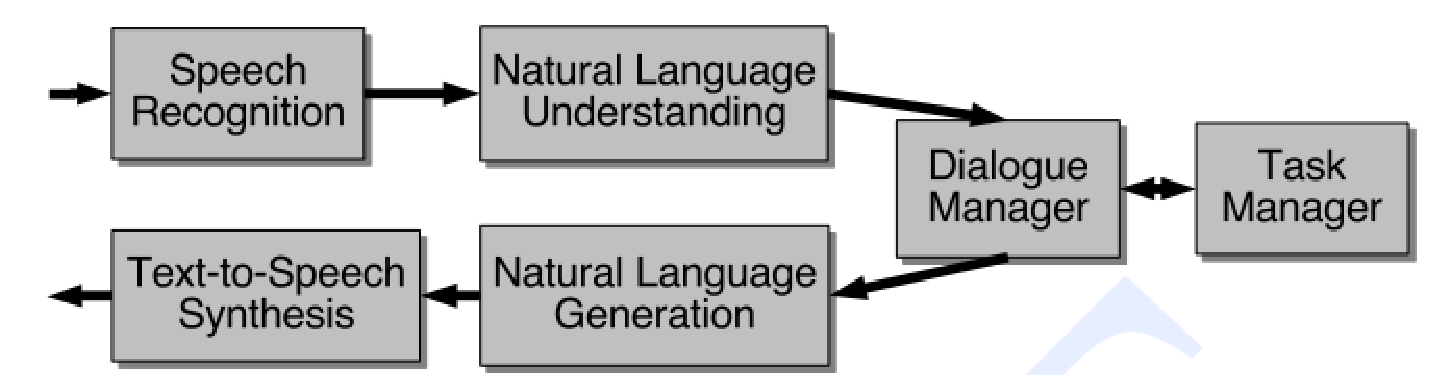
\includegraphics[width=\linewidth]{system_architecture}
  \caption{An example of system architecture}
	\label{system architecture}
\end{figure}

The following sections of this survey paper are organized as follows: From Section \ref{Automatic Speech Recognition} to Section \ref{Text-to-speech Synthesis}, we will introduce the components of goal-driven systems in further detail. Since the TM (task manager) component depends on the specific task at hand, we do not provide any paper about it. In Table \ref{tbl:system_summary}, we summary the technical details of each component used in systems that deployed in real world. We start with each of Section 2-6 a brief summary of the task of the component, and then present related previous work. Finally in Section \ref{Non-goal-driven Systems}, we present some papers about non-goal-driven systems.
